\documentclass{article}
\usepackage{ShumanNotes}

\title{Homework 1: Welcome to ECE 111}
\author{Rattanai Sawaspanich}
\date{Due October 4th @ 3 PM, 2012}
\setlength{\parindent}{0pt}
\pdfpagewidth 8.5in
\pdfpageheight 11in

\begin{document} 
\maketitle

\section{Introduction}
Welcome to ECE 111 my name is Matt Shuman and I lived in Madras, Oregon before coming to OSU for undergraduate studies in Fall 2001, and now Corvallis is home.  I am teaching three ECE courses (ECE 111, 271, and 507), taking three MBA courses (BA560\footnote{http://mime.oregonstate.edu/research/drl/}, 562, and 528), and teaching a woodworking class at the OSU craft center\footnote{http://mu.oregonstate.edu/craftcenter/}.  It's a busy term, but I'm excited for this term. Insert your image as in figure \ref{ImageLabel} using the link below and briefly introduce yourself.
\centerimage{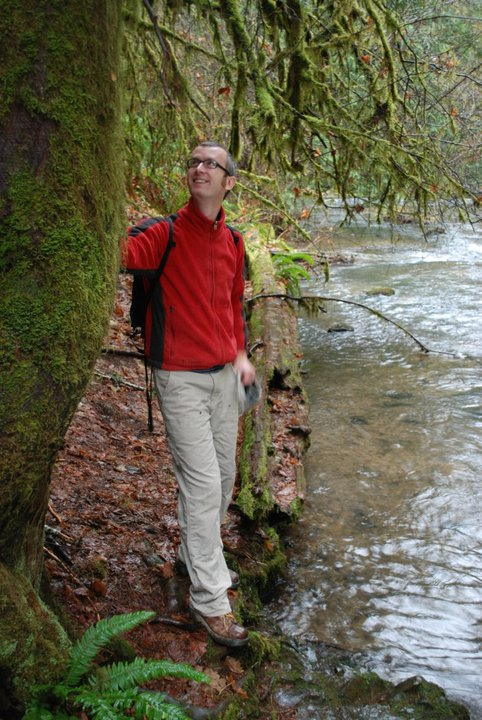
\includegraphics[width = 2in]{./HikingPicture.jpg} }{This is a caption field about the image above}{ImageLabel}\newline

\newpage
\centerimage{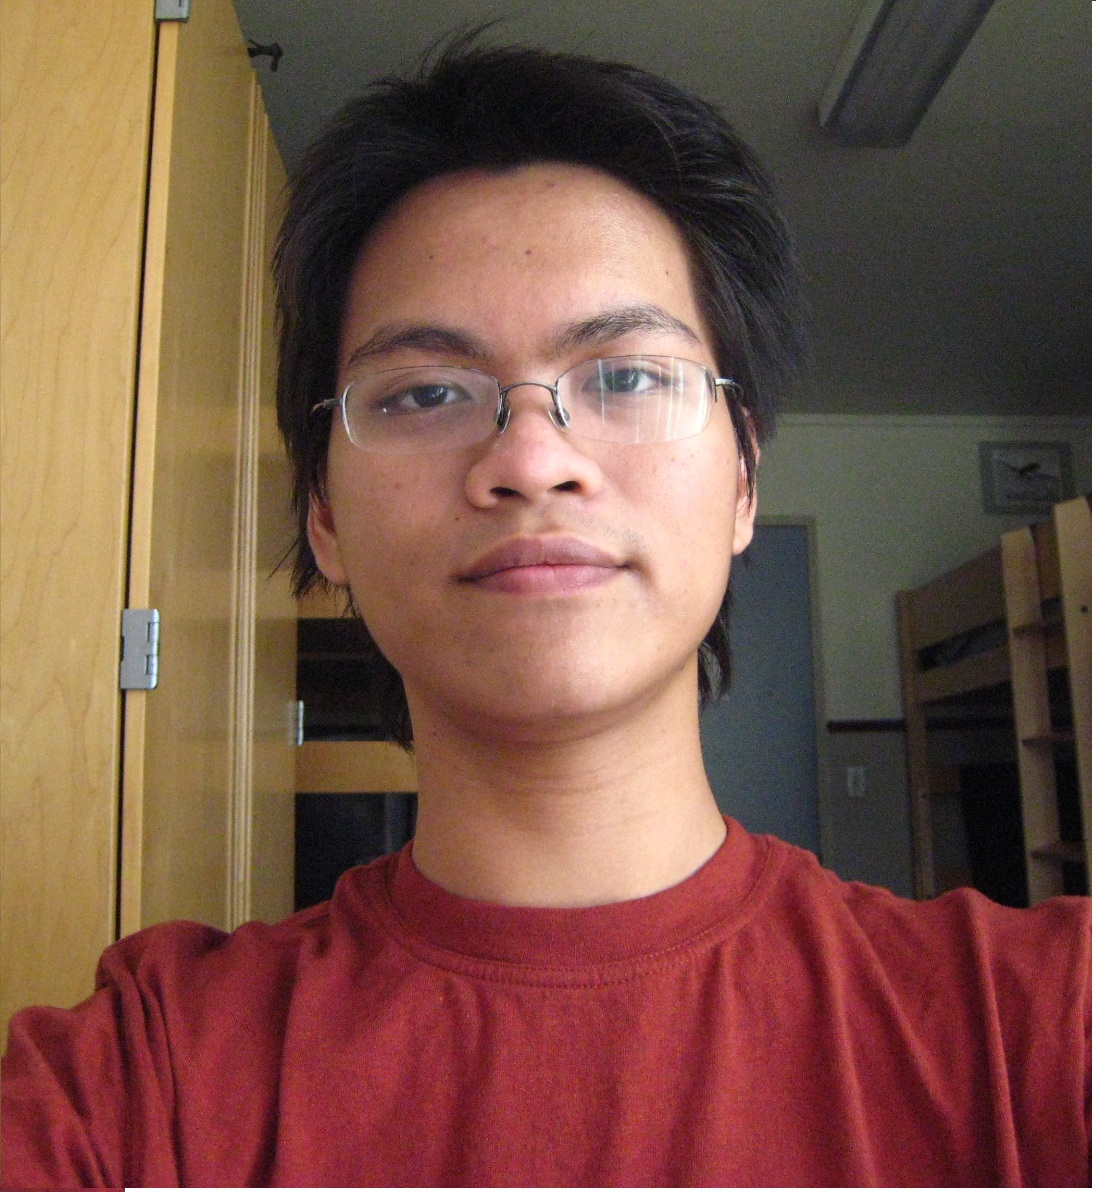
\includegraphics[width = 2in]{./IMG_0897.jpg} }{Rattanai Sawaspanich}{me}

 Hello Mr.Shuman,  My name is Rattanai Sawaspanich, but you can call me as "Bear\footnote{I picked my name as "Bear" because my \emph{nickname} in Thai is 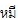
\includegraphics[width=0.115in]{./Bear_T.jpg} which means "Bear" so I translated it to English.}".  I'm from Thailand. My family own an auto-mobile garage; my dad is a mechanic and my mom helps my dad about the bussiness finance.   During my high school junior year,2010, I got accepted into AFS exchange program and was an exchange student at Shedon High School, Eugene, OR. That's how I began my student carreer in the US. After I finished my junior year, I have to transfer to Marist Catholic High School due to the J-1 VISA policy and I graduated from there. Thus, I'm a Buddhist and there were only two of us in the school ;anyhow, it was good to learn the different culture and religion.  The main reason why I chose to study in the US and go to OSU  because I want to think and make differences which is a step toward to live my legacy.  
\section{Defining Success}
\emph{Success is the achievement of something desired, planned, or attempted. After you put years and thousands of dollars into your 
college education, what do you want from your ECE degree?}
\newline\newline
What do I want from my ECE degree is the life that can live without depending on money. I'm not saying that I have to be rich. I'm saying that I can live happily and help other people beyond what money can do. I always think if I'm going to die, I would like the world to know who I am.

\section{Word Processing}
\emph{The homework assignments in ECE 111 focus on using Latex to typecast a professional looking .pdf for each assignment.  What are the advantages of Latex compared to traditional WYSIWYG \footnote{http://en.wikipedia.org/wiki/WYSIWYG} word processors?  What are the disadvantages of using Latex?}\newline\newline

It is better because \newline \begin{itemize}

\item *.pdf file can be consistently display on any devices.
\item The pdf-reciever can't actually change the information in a file.
\item Easier to format document style.
\item Smaller file size.
\end{itemize}
Anyhow, they may be some issue with Abode Reader lisence in a gray-market countries that prevent them to open .pdf file.

\section{Microcontrollers}
Atmel Microcontrollers are a very inexpensive way to develop projects.  Every future project in ECE 111 will use an Atmel Microcontroller, the Atmel Tiny26.\newline
\emph{Lookup the cost of the Tiny26 Microcontroller from Digikey}\newline
\url{http://search.digikey.com/scripts/DkSearch/dksus.dll?Detail&name=ATTINY26L-8PU-ND}.
\newline \newline
\emph{Atml Microcontroller price}\newline
\begin {center}

\begin{tabular}{|c| c| c|}
\hline
Price Break & \$ Unit Price & \$ extended Price\\
\hline
1 & 3.0600 &3.06 \\
25&1.9196&47.99\\
100&1.70640&170.64\\
\hline
\end{tabular}
\end{center}

Table formation credit: \url{http://en.wikibooks.org/wiki/LaTeX/Tables}\newline



\emph{Look up a project on Youtube that uses an Atmel Microcontroller}\newline
What does the Atmel Microcontroller do for the project you researched?\newline\newline
Here is the project I found: \url{http://www.youtube.com/watch?v=uhK0S7ZIKZ4&feature=player_embedded}\newline\newline
The Atmel Microcontroller is used as a signal converter from switchs on a chess board to become a digital signal.  Then, the digital signal was sent to be an input in a computer via a USB port. Afterward, the input were processed and ran on Fritz, a chess program, to make a move. It seems that Atmel Microcontroller is a universal microprocessor that convert on/off botton to a digital signal that can be an input to a computer via USB port. \newline
\newline
please continue next page 

\newpage
\section{Microcontroller Packages}
Integrated Circuits, ICs, are made using many different types of packages. The Tiny26 in lab is a DIP , while the 5 volt regulator is in a TO-92 package. The ECE 272 CPLD uses a 44 pin QFP. The Droid X OMAP processor is a BGA package type with over 400 pins! \newline
\newline
\emph{Insert a picture for the DIP, TO-92, QFP, and BGA package types}\newline
\newline
This link might be helpful \newline
\newline
\url{http://en.wikipedia.org/wiki/Chip_carrier}

\centering

\picsidebyside{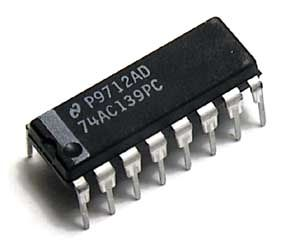
\includegraphics[width = 1 in]{./DIP.jpg}}{DIP}{DipIC}{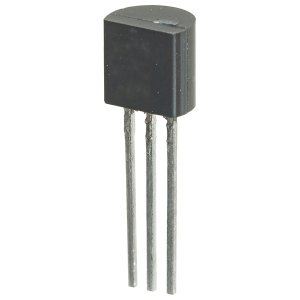
\includegraphics[width = 1 in]{./TO92.jpg}}{TO-92}{TO92} 
\picsidebyside{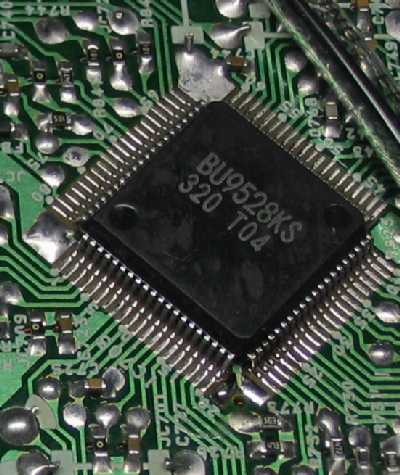
\includegraphics[width = 1 in]{./QFP.jpg}}{QFP}{QFPIC}{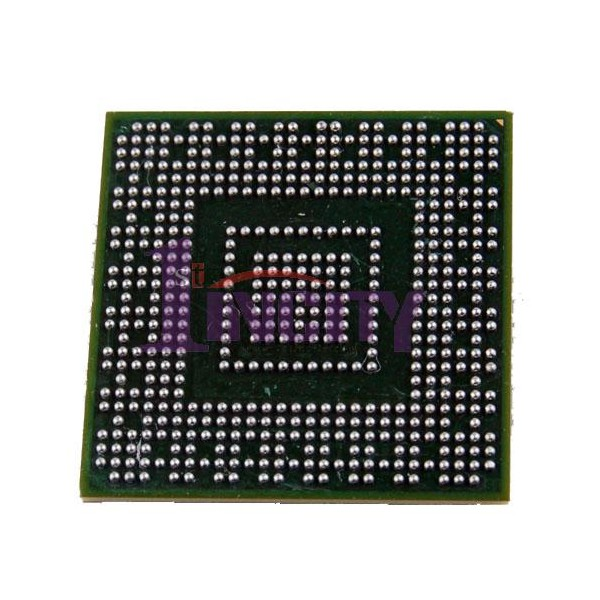
\includegraphics[width = 1 in]{./BGA.jpg}}{BGA}{BGA}





\cfoot{ECE 111 Homework \#1}

\end{document}
